%%% Local Variables:
%%% TeX-command-extra-options: "-shell-escape"
%%% mode: latex
%%% TeX-master: t
%%% End:
\documentclass{beamer}
\usepackage{caption}
\usepackage{minted}
\usepackage{tikz}
\usepackage{xcolor}
\usetikzlibrary{shapes.geometric, arrows}
\tikzstyle{startstop} = [rectangle, rounded corners, minimum width=3cm, minimum height=1cm,text centered, draw=black, fill=red!30]
\tikzstyle{io} = [trapezium, trapezium left angle=70, trapezium right angle=110, minimum width=1.5cm, minimum height=0.6cm, text centered, draw=black, fill=blue!30]
\tikzstyle{process} = [rectangle, minimum width=1.5cm, minimum height=0.5cm, text centered, draw=black, fill=orange!30]
\tikzstyle{decision} = [circle, radius=2.5cm, text centered, draw=black, fill=green!30]
\tikzstyle{arrow} = [thick,->,>=stealth]
\usepackage[labelformat=simple]{subcaption}

\usetheme{Singapore}
\title{Abstraction}

\begin{document}
\begin{frame}
\titlepage
\end{frame}
\section{Abstract Nonsense}

\begin{frame}
  \huge \centering \url{https://en.wikipedia.org/wiki/Abstract_nonsense}
\end{frame}

\begin{frame}
  \frametitle{Theories of Abstraction}
  Let's talk about abstraction.
  \begin{itemize}
  \item<2-> 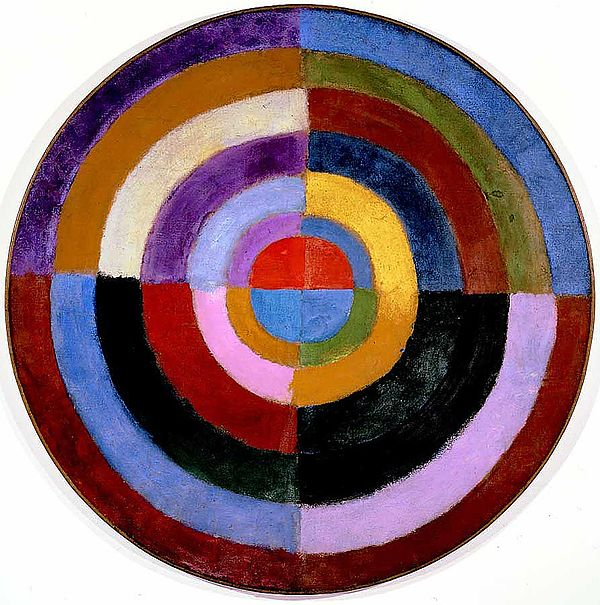
\includegraphics[width=0.3\textwidth]{images/abstract-art.jpg}
  \item<3-> Abstraction in visual
    art is about avoiding concrete subjects. It attempts
    to convey something (often an emotion) without appealing to sentiment.
  \item<4-> Oddly enough there's a bit of a stigma against it, despite the
    fact that music without lyrics has far less stigma.
  \item<5-> Abstraction in mathematics and computer science is about
    \emph{generalization}. Take away the concrete details of certain objects
    and see how they are similar.
  \end{itemize}
\end{frame}

\begin{frame}
  \frametitle{Why Abstract?}
  This can lead us to \emph{classify} different objects into
    related groups.
  \begin{itemize}
  \item<2-> Category theory has been influential in programming language theory
    because it is a powerful language for communicating abstractions in ways
    that are largely \emph{constructive}.
  \item<3-> This is important to computing because the point of programs
    are to construct some form of answer.
  \item<4-> Although categorical abstractions are powerful, I will not discuss them much (and most of the really powerful abstractions go over my head).
  \item<5-> But we will study abstraction from a less mathematical viewpoint.
  \item<6-> I will show instances of \emph{almost identical} code and how a programming language feature allows the two pieces of code to be generalized. 
  \end{itemize}    
\end{frame}

\defverbatim[colored]\buddies{
\begin{minted}[fontsize=\footnotesize]{Java}
  public boolean HasSmith(List<String> names) {
    for (String name : names) {
      if (name == "Smith")
        return true;
    }
    return false;
  }

  public  boolean HasBob(List<String> names) {
    for (String name : names) {
      if (name == "Bob")
        return true;
    }
    return false;
  }
\end{minted}
}

\begin{frame}
  \frametitle{Buddy Functions}
  Let's consider the following functions in Java:
  \buddies
  \pause
  These look pretty similar, right?
\end{frame}

\defverbatim[colored]\abstractOne{
\begin{minted}[fontsize=\footnotesize]{Java}
  public boolean HasName(String searchName, List<String> names) {
    for (String name : names) {
      if (name == searchName)
        return true;
    }
    return false;
  }
\end{minted}
}

\begin{frame}
  \frametitle{Eliminate Redundancy!}
  So, let's eliminate the redundancy of searching
  for different names by abstracting out towards
  a definition that takes in a string parameter
  to search for. This generalizes writing functions
  to search for specific strings.

  \abstractOne
  \begin{itemize}
  \item<2-> Why only design a function that searches for names?
  \item<3-> Why not search for arbitrary items so long as they
    are comparable?
  \item<4-> Then searching for names becomes an instance of a
    more general problem that is solved.    
  \end{itemize}
\end{frame}

\defverbatim[colored]\abstractTwo{
\begin{minted}[fontsize=\footnotesize]{Java}
    public <T extends Comparable<T>> boolean HasItem(T searchItem, List<T> items) {
    for (T item : items) {
      if (item.equals(searchItem))
        return true;
    }
    return false;
  }
\end{minted}
}

\begin{frame}
  \frametitle{Generic Structure}
  So, let's use some Java \emph{generics} to generalize our program.
  \abstractTwo
  \begin{itemize}
  \item<2-> Alright, now we can search for arbitrary comparable items!
  \item<3-> This is nice and general!
  \item<4-> Can we generalize any more?
  \item<5-> We actually have 2 more abstractions that we can apply!
  \end{itemize}
\end{frame}

\begin{frame}
  \frametitle{Two Abstractions??}
  \centering 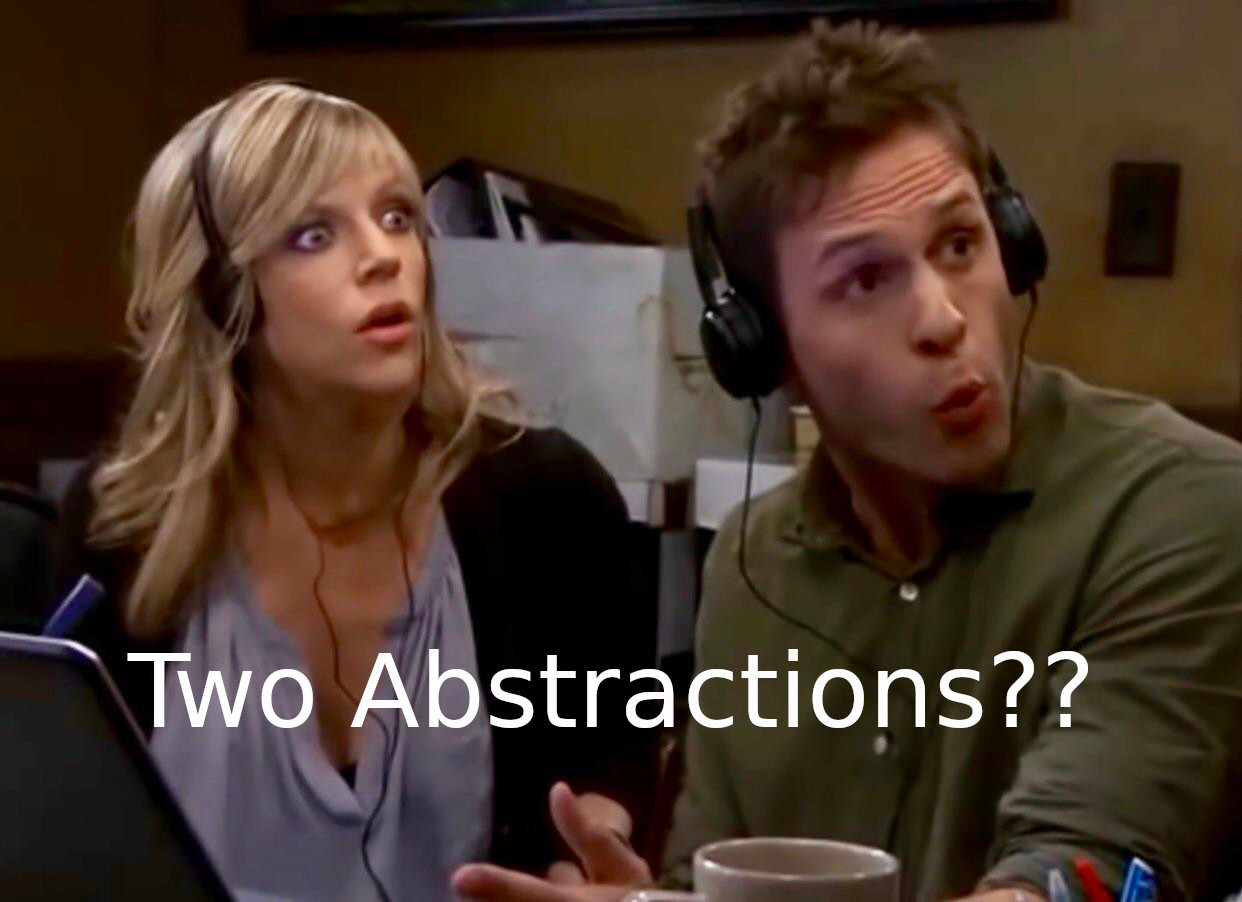
\includegraphics[width=0.6\textwidth]{images/two-abstractions.jpg}
\end{frame}

\begin{frame}
  \frametitle{I'm Sorry}
  \centering 
\includegraphics[width=0.6\textwidth]{images/unnecessary.png}
\end{frame}

\defverbatim[colored]\abstractThree{
\begin{minted}[fontsize=\footnotesize]{Java}
    public <T extends Comparable<T>> boolean TestItems(Predicate<T> pred, List<T> items) {
    for (T item : items) {
      if (pred.test(searchItem))
        return true;
    }
    return false;
  }
\end{minted}
}

\begin{frame}
  \frametitle{Back on Track}
  Ok, let's get down to business.
  \begin{itemize}
  \item<2-> 
\includegraphics[width=0.3\textwidth]{images/business.png}
  \item<3-> We can actually consider searching for a specific item via equality
    as the process of seeing if an arbitrary predicate returns true for an item
    in a list.
  \item<4-> So if we wanted to check if a string equaled smith we could write:
    \mintinline{Java}{Predicate<String> isSmith = str -> str == "Smith";}
  \item<5-> I could then pass this as the first argument to a funciton \mintinline{Java}{TestItems}
    that I will now define.
  \end{itemize}
\end{frame}

\defverbatim[colored]\abstractFour{
\begin{minted}[fontsize=\footnotesize]{Java}
    public <T extends Comparable<T>> boolean TestItems(Predicate<T> pred, Iterable<T> items) {
    for (T item : items) {
      if (pred.test(searchItem))
        return true;
    }
    return false;
  }
\end{minted}
}

\begin{frame}
  \frametitle{Last Abstraction}
  Here is that function now:
  \abstractThree
  \begin{itemize}
  \item<2-> We can provide one last abstraction that applies predicates to every item in \emph{any iterable collection}.
  \item<3-> For example, if I define iterators over dictionaries or trees we should still be able to
    apply a predicate to them.
  \item<4-> \abstractFour
  \end{itemize}
\end{frame}

\end{document}
%%% Local Variables:
%%% TeX-command-extra-options: "-shell-escape"
%%% mode: latex
%%% TeX-master: t
%%% End:
